\documentclass[english, 11 pt, class=article, crop=false]{standalone}

% note
\newcommand{\note}{Note}
\newcommand{\notesm}[1]{{\footnotesize \textsl{\note:} #1}}
\newcommand{\selos}{See the solutions manual.}

\newcommand{\texandasy}{The text is written in \LaTeX\ and the figures are made with the aid of Asymptote.}

\newcommand{\ekstitle}{Example }
\newcommand{\sprtitle}{The language box}
\newcommand{\expl}{explanation}

%%% SECTION HEADLINES %%%

% Our numbers
\newcommand{\likteikn}{The equal sign}
\newcommand{\talsifverd}{Numbers, digits and values}
\newcommand{\koordsys}{Coordinate systems}

% Calculations
\newcommand{\adi}{Addition}
\newcommand{\sub}{Subtraction}
\newcommand{\gong}{Multiplication}
\newcommand{\del}{Division}

%Factorization and order of operations
\newcommand{\fak}{Factorization}
\newcommand{\rrek}{Order of operations}

%Fractions
\newcommand{\brgrpr}{Introduction}
\newcommand{\brvu}{Values, expanding and simplifying}
\newcommand{\bradsub}{Addition and subtraction}
\newcommand{\brgngheil}{Fractions multiplied by integers}
\newcommand{\brdelheil}{Fractions divided by integers}
\newcommand{\brgngbr}{Fractions multiplied by fractions}
\newcommand{\brkans}{Cancelation of fractions}
\newcommand{\brdelmbr}{Division by fractions}
\newcommand{\Rasjtal}{Rational numbers}

%Negative numbers
\newcommand{\negintro}{Introduction}
\newcommand{\negrekn}{The elementary operations}
\newcommand{\negmeng}{Negative numbers as amounts}

%Calculation methods
\newcommand{\delmedtihundre}{Deling med 10, 100, 1\,000 osv.}

% Geometry 1
\newcommand{\omgr}{Terms}
\newcommand{\eignsk}{Attributes of triangles and quadrilaterals}
\newcommand{\omkr}{Perimeter}
\newcommand{\area}{Area}

%Algebra 
\newcommand{\algintro}{Introduction}
\newcommand{\pot}{Powers}
\newcommand{\irrasj}{Irrational numbers}

%Equations
\newcommand{\ligintro}{Introduction}
\newcommand{\liglos}{Solving with the elementary operations}
\newcommand{\ligloso}{Solving with elementary operations summarized}

%Functions
\newcommand{\fintro}{Introduction}
\newcommand{\lingraf}{Linear functions and graphs}

%Geometry 2
\newcommand{\geoform}{Formulas of area and perimeter}
\newcommand{\kongogsim}{Congruent and similar triangles}
\newcommand{\geofork}{Explanations}

% Names of rules
\newcommand{\adkom}{Addition is commutative}
\newcommand{\gangkom}{Multiplication is commutative}
\newcommand{\brdef}{Fractions as rewriting of division}
\newcommand{\brtbr}{Fractions multiplied by fractions}
\newcommand{\delmbr}{Fractions divided by fractions}
\newcommand{\gangpar}{Distributive law}
\newcommand{\gangparsam}{Paranthesis multiplied together}
\newcommand{\gangmnegto}{Multiplication by negative numbers I}
\newcommand{\gangmnegtre}{Multiplication by negative numbers II}
\newcommand{\konsttre}{Unique construction of triangles}
\newcommand{\kongtre}{Congruent triangles}
\newcommand{\topv}{Vertical angles}
\newcommand{\trisum}{The sum of angles in a triangle}
\newcommand{\firsum}{The sum of angles in a quadrilateral}
\newcommand{\potgang}{Multiplication by powers}
\newcommand{\potdivpot}{Division by powers}
\newcommand{\potanull}{The special case of \boldmath $a^0$}
\newcommand{\potneg}{Powers with negative exponents}
\newcommand{\potbr}{Fractions as base}
\newcommand{\faktgr}{Factors as base}
\newcommand{\potsomgrunn}{Powers as base}
\newcommand{\arsirk}{The area of a circle}
\newcommand{\artrap}{The area of a trapezoid}
\newcommand{\arpar}{The area of a parallelogram}
\newcommand{\pyt}{Pythagoras's theorem}
\newcommand{\forform}{Ratios in similar triangles}
\newcommand{\vilkform}{Terms of similar triangles}
\newcommand{\omkrsirk}{The perimeter of a circle (and the value of $ \bm \pi $)}
\newcommand{\artri}{The area of a triangle}
\newcommand{\arrekt}{The area of a rectangle}
\newcommand{\liknflyt}{Moving terms across the equal sign}
\newcommand{\funklin}{Linear functions}


\usepackage[T1]{fontenc}
%\renewcommand*\familydefault{\sfdefault} % For dyslexia-friendly text
\usepackage{lmodern} % load a font with all the characters
\usepackage{geometry}
\geometry{verbose,paperwidth=16.1 cm, paperheight=24 cm, inner=2.3cm, outer=1.8 cm, bmargin=2cm, tmargin=1.8cm}
\setlength{\parindent}{0bp}
\usepackage{import}
\usepackage[subpreambles=false]{standalone}
\usepackage{amsmath}
\usepackage{amssymb}
\usepackage{esint}
\usepackage{babel}
\usepackage{tabu}
\makeatother
\makeatletter

\usepackage{titlesec}
\usepackage{ragged2e}
\RaggedRight
\raggedbottom
\frenchspacing

% Norwegian names of figures, chapters, parts and content
\addto\captionsenglish{\renewcommand{\figurename}{Figur}}
\makeatletter
\addto\captionsenglish{\renewcommand{\chaptername}{Kapittel}}
\addto\captionsenglish{\renewcommand{\partname}{Del}}


\usepackage{graphicx}
\usepackage{float}
\usepackage{subfig}
\usepackage{placeins}
\usepackage{cancel}
\usepackage{framed}
\usepackage{wrapfig}
\usepackage[subfigure]{tocloft}
\usepackage[font=footnotesize,labelfont=sl]{caption} % Figure caption
\usepackage{bm}
\usepackage[dvipsnames, table]{xcolor}
\definecolor{shadecolor}{rgb}{0.105469, 0.613281, 1}
\colorlet{shadecolor}{Emerald!15} 
\usepackage{icomma}
\makeatother
\usepackage[many]{tcolorbox}
\usepackage{multicol}
\usepackage{stackengine}

\usepackage{esvect} %For vectors with capital letters

% For tabular
\usepackage{array}
\usepackage{multirow}
\usepackage{longtable} %breakable table

% Ligningsreferanser
\usepackage{mathtools}
\mathtoolsset{showonlyrefs}

% index
\usepackage{imakeidx}
\makeindex[title=Indeks]

%Footnote:
\usepackage[bottom, hang, flushmargin]{footmisc}
\usepackage{perpage} 
\MakePerPage{footnote}
\addtolength{\footnotesep}{2mm}
\renewcommand{\thefootnote}{\arabic{footnote}}
\renewcommand\footnoterule{\rule{\linewidth}{0.4pt}}
\renewcommand{\thempfootnote}{\arabic{mpfootnote}}

%colors
\definecolor{c1}{cmyk}{0,0.5,1,0}
\definecolor{c2}{cmyk}{1,0.25,1,0}
\definecolor{n3}{cmyk}{1,0.,1,0}
\definecolor{neg}{cmyk}{1,0.,0.,0}

% Lister med bokstavar
\usepackage[inline]{enumitem}

\newcounter{rg}
\numberwithin{rg}{chapter}
\newcommand{\reg}[2][]{\begin{tcolorbox}[boxrule=0.3 mm,arc=0mm,colback=blue!3] {\refstepcounter{rg}\phantomsection \large \textbf{\therg \;#1} \vspace{5 pt}}\newline #2  \end{tcolorbox}\vspace{-5pt}}

\newcommand\alg[1]{\begin{align} #1 \end{align}}

\newcommand\eks[2][]{\begin{tcolorbox}[boxrule=0.3 mm,arc=0mm,enhanced jigsaw,breakable,colback=green!3] {\large \textbf{Eksempel #1} \vspace{5 pt}\\} #2 \end{tcolorbox}\vspace{-5pt} }

\newcommand{\st}[1]{\begin{tcolorbox}[boxrule=0.0 mm,arc=0mm,enhanced jigsaw,breakable,colback=yellow!12]{ #1} \end{tcolorbox}}

\newcommand{\spr}[1]{\begin{tcolorbox}[boxrule=0.3 mm,arc=0mm,enhanced jigsaw,breakable,colback=yellow!7] {\large \textbf{Språkboksen} \vspace{5 pt}\\} #1 \end{tcolorbox}\vspace{-5pt} }

\newcommand{\sym}[1]{\colorbox{blue!15}{#1}}

\newcommand{\info}[2]{\begin{tcolorbox}[boxrule=0.3 mm,arc=0mm,enhanced jigsaw,breakable,colback=cyan!6] {\large \textbf{#1} \vspace{5 pt}\\} #2 \end{tcolorbox}\vspace{-5pt} }

\newcommand\algv[1]{\vspace{-11 pt}\begin{align*} #1 \end{align*}}

\newcommand{\regv}{\vspace{5pt}}
\newcommand{\mer}{\textsl{Merk}: }
\newcommand{\mers}[1]{{\footnotesize \mer #1}}
\newcommand\vsk{\vspace{11pt}}
\newcommand\vs{\vspace{-11pt}}
\newcommand\vsb{\vspace{-16pt}}
\newcommand\sv{\vsk \textbf{Svar} \vspace{4 pt}\\}
\newcommand\br{\\[5 pt]}
\newcommand{\figp}[1]{../fig/#1}
\newcommand\algvv[1]{\vs\vs\begin{align*} #1 \end{align*}}
\newcommand{\y}[1]{$ {#1} $}
\newcommand{\os}{\\[5 pt]}
\newcommand{\prbxl}[2]{
\parbox[l][][l]{#1\linewidth}{#2
	}}
\newcommand{\prbxr}[2]{\parbox[r][][l]{#1\linewidth}{
		\setlength{\abovedisplayskip}{5pt}
		\setlength{\belowdisplayskip}{5pt}	
		\setlength{\abovedisplayshortskip}{0pt}
		\setlength{\belowdisplayshortskip}{0pt} 
		\begin{shaded}
			\footnotesize	#2 \end{shaded}}}

\renewcommand{\cfttoctitlefont}{\Large\bfseries}
\setlength{\cftaftertoctitleskip}{0 pt}
\setlength{\cftbeforetoctitleskip}{0 pt}

\newcommand{\bs}{\\[3pt]}
\newcommand{\vn}{\\[6pt]}
\newcommand{\fig}[1]{\begin{figure}
		\centering
		\includegraphics[]{\figp{#1}}
\end{figure}}

\newcommand{\figc}[2]{\begin{figure}
		\centering
		\includegraphics[]{\figp{#1}}
		\caption{#2}
\end{figure}}

\newcommand{\sectionbreak}{\clearpage} % New page on each section

\newcommand{\nn}[1]{
\begin{equation}
	#1
\end{equation}
}

% Equation comments
\newcommand{\cm}[1]{\llap{\color{blue} #1}}

\newcommand\fork[2]{\begin{tcolorbox}[boxrule=0.3 mm,arc=0mm,enhanced jigsaw,breakable,colback=yellow!7] {\large \textbf{#1 (forklaring)} \vspace{5 pt}\\} #2 \end{tcolorbox}\vspace{-5pt} }
 
%colors
\newcommand{\colr}[1]{{\color{red} #1}}
\newcommand{\colb}[1]{{\color{blue} #1}}
\newcommand{\colo}[1]{{\color{orange} #1}}
\newcommand{\colc}[1]{{\color{cyan} #1}}
\definecolor{projectgreen}{cmyk}{100,0,100,0}
\newcommand{\colg}[1]{{\color{projectgreen} #1}}

% Methods
\newcommand{\metode}[2]{
	\textsl{#1} \\[-8pt]
	\rule{#2}{0.75pt}
}

%Opg
\newcommand{\abc}[1]{
	\begin{enumerate}[label=\alph*),leftmargin=18pt]
		#1
	\end{enumerate}
}
\newcommand{\abcs}[2]{
	\begin{enumerate}[label=\alph*),start=#1,leftmargin=18pt]
		#2
	\end{enumerate}
}
\newcommand{\abcn}[1]{
	\begin{enumerate}[label=\arabic*),leftmargin=18pt]
		#1
	\end{enumerate}
}
\newcommand{\abch}[1]{
	\hspace{-2pt}	\begin{enumerate*}[label=\alph*), itemjoin=\hspace{1cm}]
		#1
	\end{enumerate*}
}
\newcommand{\abchs}[2]{
	\hspace{-2pt}	\begin{enumerate*}[label=\alph*), itemjoin=\hspace{1cm}, start=#1]
		#2
	\end{enumerate*}
}

% Oppgaver
\newcommand{\opgt}{\phantomsection \addcontentsline{toc}{section}{Oppgaver} \section*{Oppgaver for kapittel \thechapter}\vs \setcounter{section}{1}}
\newcounter{opg}
\numberwithin{opg}{section}
\newcommand{\op}[1]{\vspace{15pt} \refstepcounter{opg}\large \textbf{\color{blue}\theopg} \vspace{2 pt} \label{#1} \\}
\newcommand{\ekspop}[1]{\vsk\textbf{Gruble \thechapter.#1}\vspace{2 pt} \\}
\newcommand{\nes}{\stepcounter{section}
	\setcounter{opg}{0}}
\newcommand{\opr}[1]{\vspace{3pt}\textbf{\ref{#1}}}
\newcommand{\oeks}[1]{\begin{tcolorbox}[boxrule=0.3 mm,arc=0mm,colback=white]
		\textit{Eksempel: } #1	  
\end{tcolorbox}}
\newcommand\opgeks[2][]{\begin{tcolorbox}[boxrule=0.1 mm,arc=0mm,enhanced jigsaw,breakable,colback=white] {\footnotesize \textbf{Eksempel #1} \\} \footnotesize #2 \end{tcolorbox}\vspace{-5pt} }
\newcommand{\rknut}{
Rekn ut.
}

%License
\newcommand{\lic}{\textit{Matematikken sine byggesteinar by Sindre Sogge Heggen is licensed under CC BY-NC-SA 4.0. To view a copy of this license, visit\\ 
		\net{http://creativecommons.org/licenses/by-nc-sa/4.0/}{http://creativecommons.org/licenses/by-nc-sa/4.0/}}}

%referances
\newcommand{\net}[2]{{\color{blue}\href{#1}{#2}}}
\newcommand{\hrs}[2]{\hyperref[#1]{\color{blue}\textsl{#2 \ref*{#1}}}}
\newcommand{\rref}[1]{\hrs{#1}{regel}}
\newcommand{\refkap}[1]{\hrs{#1}{kapittel}}
\newcommand{\refsec}[1]{\hrs{#1}{seksjon}}

\newcommand{\mb}{\net{https://sindrsh.github.io/FirstPrinciplesOfMath/}{MB}}


%line to seperate examples
\newcommand{\linje}{\rule{\linewidth}{1pt} }

\usepackage{datetime2}
%%\usepackage{sansmathfonts} for dyslexia-friendly math
\usepackage[]{hyperref}



\begin{document}
\section{GeoGebra}
\subsection{Introduction}
When you open GeoGebra, you see a picture like this:
\begin{figure}[H]
	\centering
	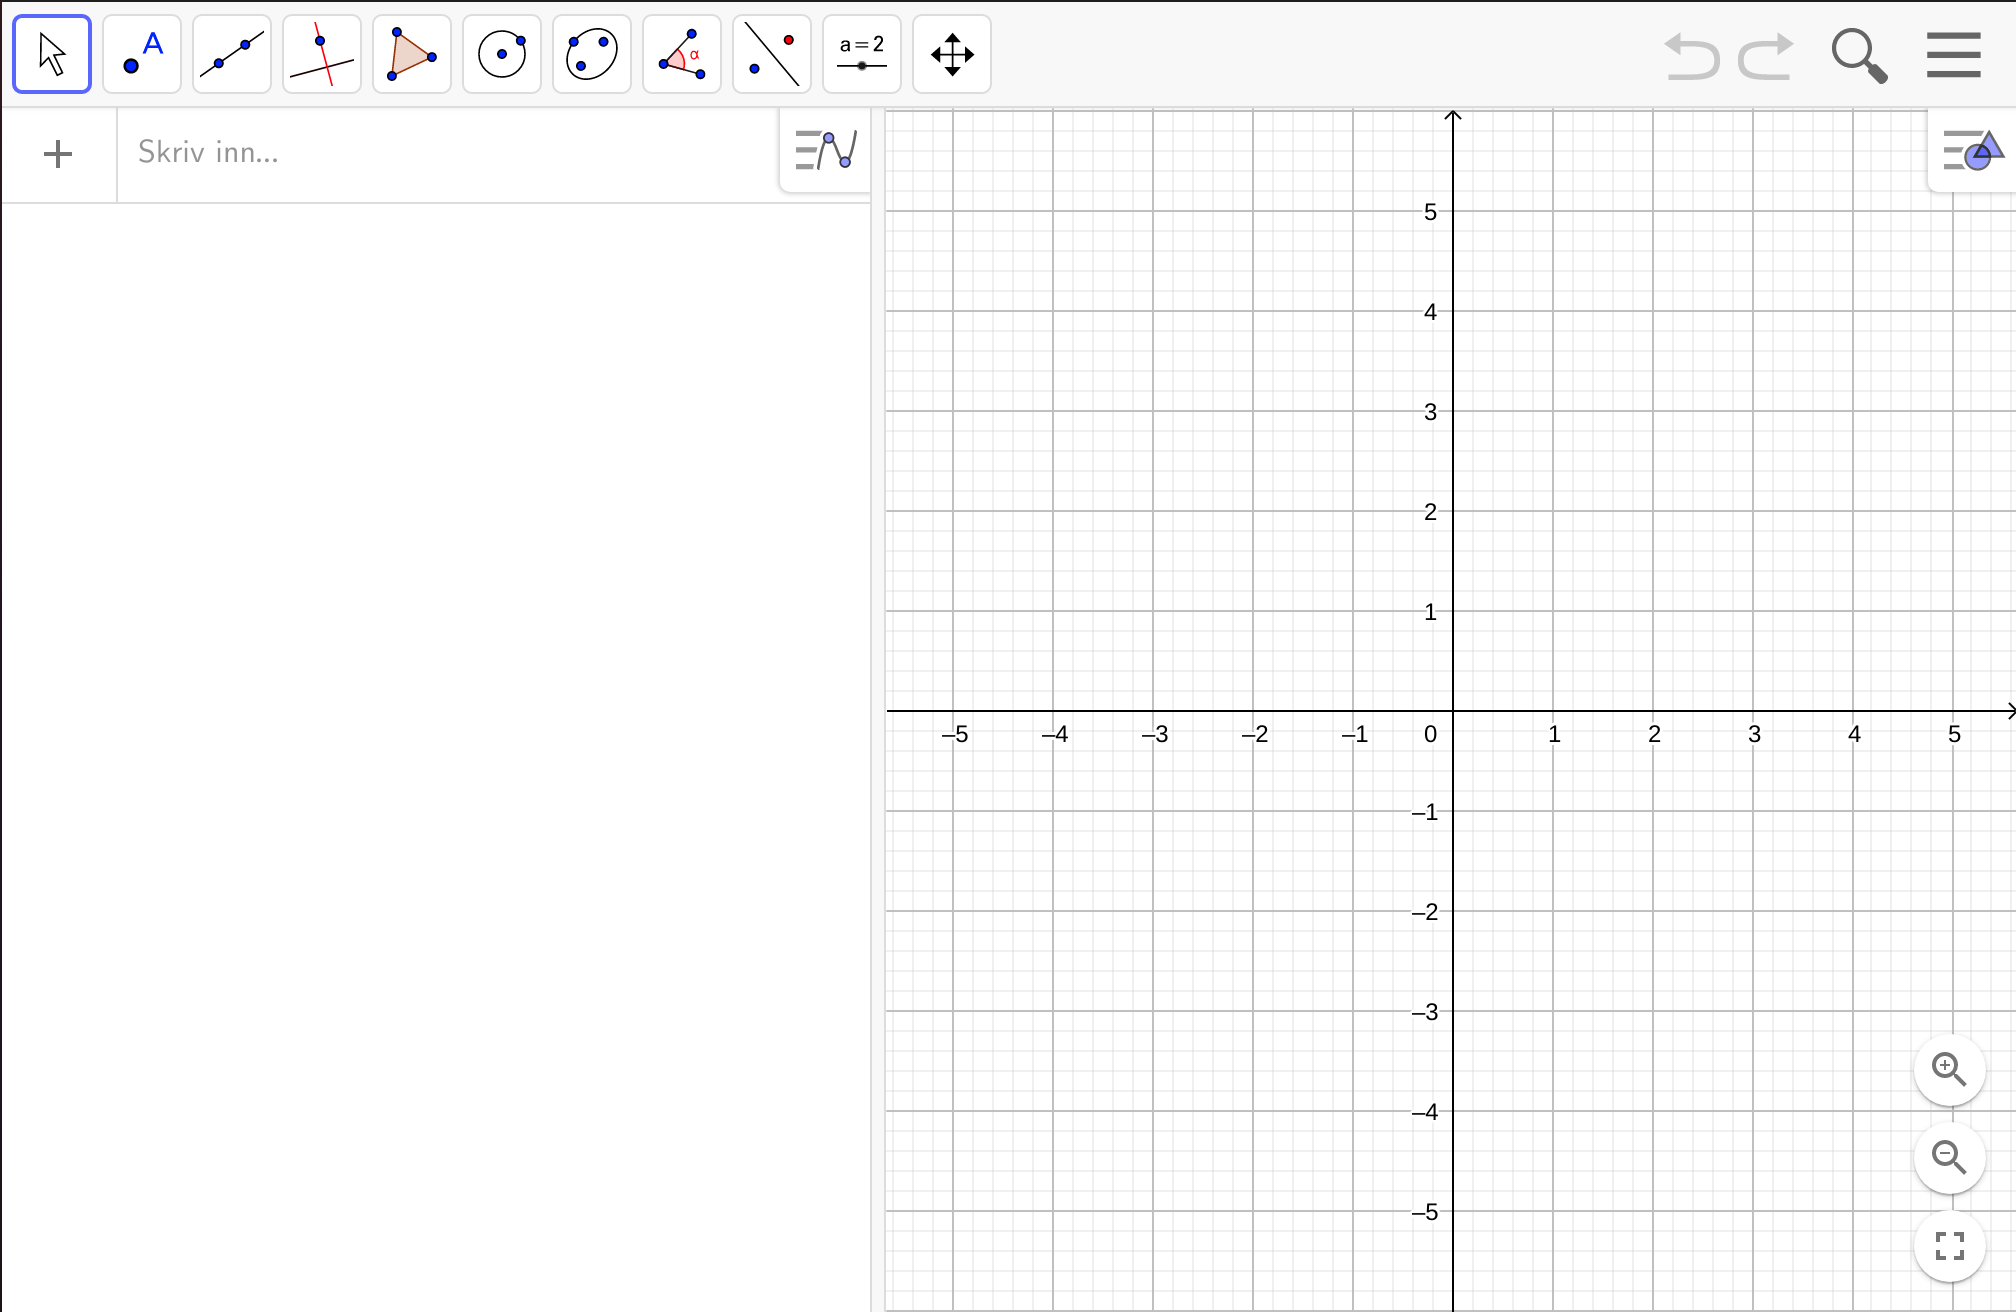
\includegraphics[scale=0.1]{ggbalgoggraf}
\end{figure}
The field labeled "Skriv inn" is called the \textit{input field}. This field, along with the blank field below, constitutes the \textit{algebra field}. The coordinate system on the right is called the \textit{graphics field}.

\subsection{Entering points, functions, and lines}
\subsubsection{Points}
Suppose we want the points $ (1,3) $ and $ (4,5) $ to appear in the graphics field. In the input field, we then write
\g{(1,3)}
and \vs
\g{(4,5)}
GeoGebra then names the points $ A $ and $ B $, and plots them in the graphics field:
\begin{figure}[H]
	\centering
	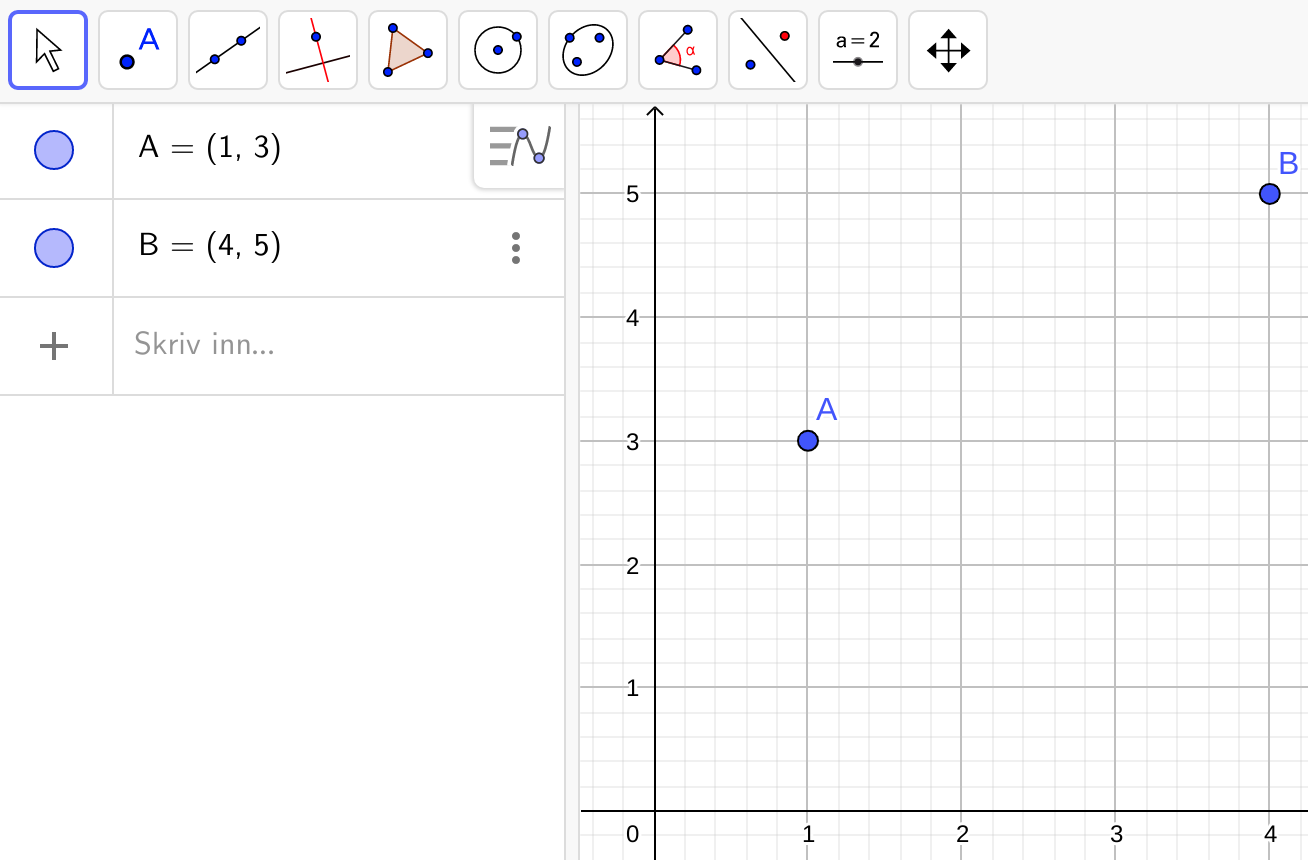
\includegraphics[scale=0.15]{pointAandB}
\end{figure}
If we want to set a point's name ourselves, we can write, for instance,
\g{P=(2,4)}
\begin{figure}[H]
	\centering
	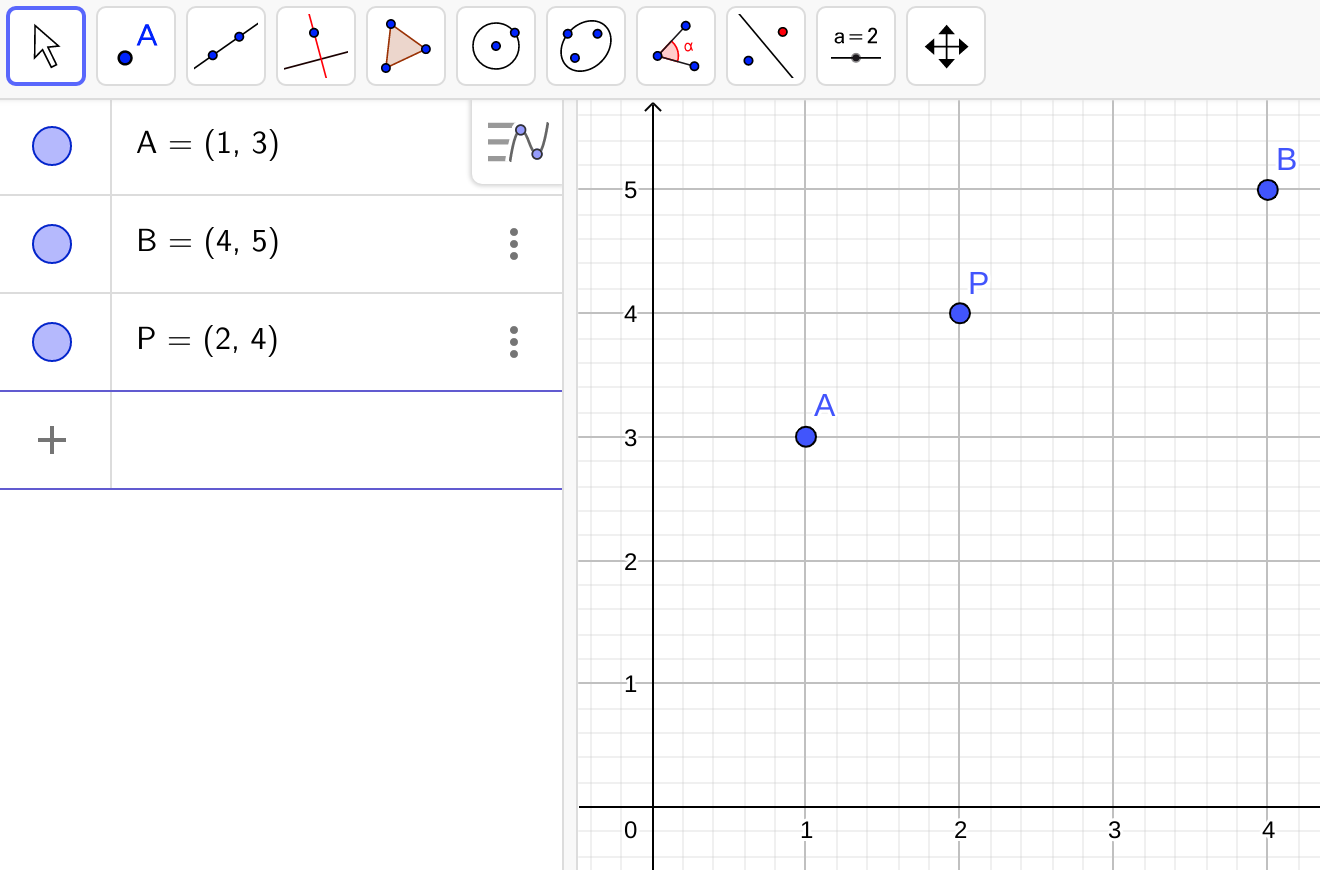
\includegraphics[scale=0.15]{pointP}
\end{figure}
\subsubsection{Functions}
Suppose we have the function 
\[f(x)= \frac{3}{2} x^2 + 3x \]
To use $ f(x) $ in GeoGebra, we write:
\g{3/2*x\^{}2+3x}
When we do not give the function a name, GeoGebra will automatically name the function $ f $. In the algebra field, we therefore get
\begin{figure}[H]
	\centering
	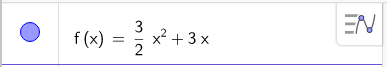
\includegraphics[scale=0.5]{skrivf}
\end{figure}
In the graphics field, we get the graph of $ f $. \vsk

If instead we have the function
\[ P(x)= 0.15x^3 - 0.4 x\]
there are two things to be aware of. The first is that \textsl{all decimals must be written using a period instead of a comma} in GeoGebra. The second is that we want to give the function the name $ P(x) $. We then write
\g{P(x) = 0.15x\^{}3 - 0.4x}
and get \vspace{-5pt}
\begin{figure}[H]
	\centering
	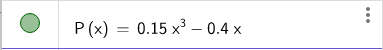
\includegraphics[scale=0.5]{pfig}
\end{figure}
\info{Note!}{
	You can never name functions $ {y(x)} $ in GeoGebra. $ y $ can only be used when entering expressions for a straight line, i.e., $ {y=ax +b} $, where $ a $ and $ b $ are two arbitrary numbers.
}

\subsubsection{Horizontal and Vertical Lines}

If we want to create a line that runs horizontally through the value 3 on the \(y\)-axis and a line that runs vertically through the value 2 on the \(x\)-axis, we write:
\g{y = 3}
and 
\g{x = 2 }
This gives us the following figure:
\begin{figure}[H]
	\centering
	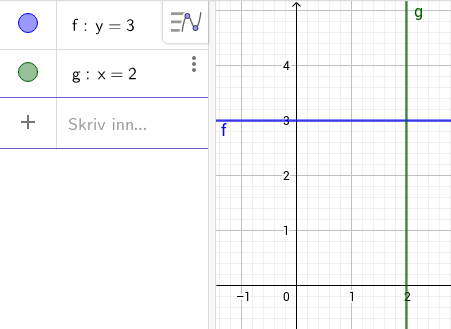
\includegraphics[scale=0.5]{23}
\end{figure}

\subsection{Finding the Value of Functions and Lines}
\subsubsection{Functions}
Suppose we have the function
\[H(x) = x^2 + 3x -3 \]
If we want to know what \(H(2)\) is, we write:
\g{H(2)}
which results in this:
\begin{figure}[H]
	\centering
	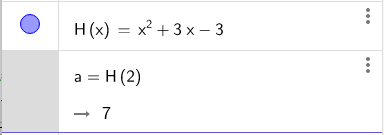
\includegraphics[scale=0.5]{H}
\end{figure}
From this, we know that \(H(2) = 7\).
\subsubsection{Lines}
It is strongly recommended that you use function expressions when dealing with lines in GeoGebra, but in some cases, you cannot avoid lines in the form \(y = ax + b\). \vsk

Consider the two lines \vs
\alg{
	y &= x-3 \vn
	y &= -2x+1
}
We enter these into GeoGebra, and get:
\begin{figure}[H]
	\centering
	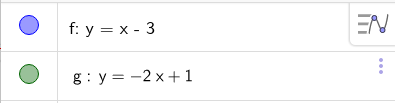
\includegraphics[scale=0.5]{fglin1}
\end{figure}
If we now want to find out what the value of \(y = x-3\) is when \(x = 2\), we need to note that GeoGebra has named this line \(f\). The answer we are looking for is then obtained by writing \(f(2)\). If we also want to know what \(y = -2x+1\) is when \(x = 0\), we write \(g(0)\):
\begin{figure}[H]
	\centering
	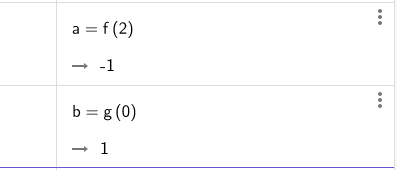
\includegraphics[scale=0.6]{fglin2}
\end{figure}


\newpage
\subsection{Buttons and Commands}

\subsubsection*{Graphics Field}
Buttons are selected from dropdown menus on the toolbar. The numbering of the menus is from the left.\vsk

\begin{tabular}{@{}l}
	\,
\includegraphics[scale=0.4]{fig/pkt} Creates a new point. (Menu no. 1) \\
	\,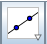
\includegraphics[scale=0.4]{fig/lin} Creates a line between two points. (Menu no. 2)\\	
	\,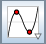
\includegraphics[scale=0.4]{fig/ekst} Finds the maximum and minimum points of a function. (Menu no. 2)\\
	\,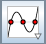
\includegraphics[scale=0.4]{fig/nul} Finds the zeros of a function. (Menu no. 2)	\\
	\,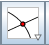
\includegraphics[scale=0.4]{fig/skj} Finds the intersection point between two objects. (Menu no. 3)\\	
	\,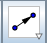
\includegraphics[scale=0.4]{fig/vek} Creates the vector between two points (Menu no. 3)\\		
	\,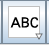
\includegraphics[scale=0.4]{fig/tekst} Creates a text box. (Menu no. 10)\\		
	\,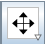
\includegraphics[scale=0.4]{fig/flytt} Moves the graphics field. Changes the value distance if pointing at the axes. \\
	\hspace{1cm}(Menu no. 10)\\			
\end{tabular}

\subsubsection{Shortcut Keys}
\begin{tabular}{@{}c | c |c | c }
	&\textbf{Description} & \textbf{PC }& \textbf{Mac} \\ \hline
	$ \sqrt{} $	& square root& \texttt{alt\,+\,r} &\texttt{alt\,+\,r} \\\hline
	$ \pi $	& pi& \texttt{alt\,+\,p} & \texttt{alt\,+\,p}\\\hline
	$ \infty $ &infinity& \texttt{alt\,+\,u} &\texttt{alt\,+\,,}  \\\hline
	$ \otimes $&cross product & \texttt{alt\,+\,shift\,+\,8}&\texttt{ctrl\,+\,shift\,+\,8} \\\hline
	$ e $&euler's number & \texttt{alt\,+\,e}& \texttt{alt\,+\,e}\\\hline
	$ {}^\circ $&degree symbol ($ \frac{\pi}{180} $) & \texttt{alt\,+\,o}& \texttt{alt\,+\,o}
	\\\hline	
\end{tabular}
\newpage

\subsubsection{Videos}
\begin{itemize}
	\item \net{https://drive.google.com/file/d/1u9u6eZFW8yqtM2ukdW9716i1_YH0NMOa/view?usp=sharing}{Find the zeros of a graph}
	\item \net{https://drive.google.com/file/d/11B7o3WMrbR5cpfshkv9FSBpQ5khBCwLS/view?usp=sharing}{Find the local minimum (or maximum) of a graph}
	\item \net{https://drive.google.com/file/d/1koy-ffEejtIt-YbIohoFN4gbMLi-95cb/view?usp=sharing}{Find the intersection points of two functions}
	\item \net{https://drive.google.com/file/d/1Z8v05XjlqsSFpHEed5q4s0nGDjdQUfqs/view?usp=sharing}{Adjust axes}
	\item \net{https://drive.google.com/file/d/1oKKDk084IEhy11rNhDk0-VykzXLuhthy/view?usp=sharing}{Change thickness, color, etc. on graph}
	\item \net{https://drive.google.com/file/d/1568rRj2PxzwK6wSm7v4w3GWzDnGtSuuX/view?usp=sharing}{Draw graph on a given interval} \\
	{\footnotesize In the video, we draw \(f(x)= x^2-3x+2\) on the interval \(0 \leq x \leq 5\)}.
	\item \net{https://drive.google.com/file/d/1x7y7DJMJ-7rfpgapB48e5Nlq6UnXXcI2/view?usp=sharing}{Draw a line between two points} \\
	{\footnotesize Notice what is done towards the end of the video to get the familiar expression \(y=ax+b\)}.
	\item \net{https://drive.google.com/file/d/18cNeX3vJFEY7BpgrH_BFpI1q4c-bczyH/view?usp=sharing}{Perform regression}\\
	{\footnotesize In the video, we have previously entered the numbers in the table below, which shows the electric car sales in Norway the number of years after 2010. These numbers were also used in \refsec{Regression}. \os
		Regression is performed with a line, a quadratic function, and a 4th-degree function.
		
		\begin{tabular}{c|c}
			\textbf{number of years} & \textbf{electric cars} \\ \hline
			0 &	3347\\
			1 &	5381\\
			2 &	9565\\
			3 &	19678\\
			4 &	42356\\
			5 &	73312\\
			6 &	101126\\
			7 &	138477\\
			8 &	194900\\
			9 &	260688\\
			10 &337201\\
			11 &	455271\\
		\end{tabular}
	}
\end{itemize}

\newpage
\subsubsection{Command List}
\mers{Many of the commands have their own buttons, as shown in the videos above.}
\begin{itemize}
	\item \cmds{abs( <x> )}{Gives the length of \( x \) (a number, a line segment, etc.). Alternatively, you can write {\tt{|x|}}}.
	
	\item \cmds{Line( <Point>, <Point> )}{Gives the line between two points.}
	
	\item \cmds{ExtremalPoint( <Function>, <Start>, <End> )}{Finds local maxima and minima for a function over a specified interval.}
	
	\item \cmds{Function( <Function>, <Start>, <End> )}{Draws a function within a specified interval.}
	
	\item \cmds{Polygon( <Point>, ..., <Point> )}{Draws the polygon between the given points.}
	
	\item \cmds{Zeroes( <Function>, <Start>, <End> )}{Provides the zeroes of a function within a specified interval.}
	
	\item \cmds{LinReg( <List> )}
	{Uses linear regression to fit points given in a list.}
	
	\item \cmds{ExpReg( <List> )}
	{Uses regression with an exponential function to fit points given in a list.}
	
	\item \cmds{PolyReg( <List>, <Degree> )}
	{Uses regression with a polynomial of a given degree to fit points provided in a list.}
	
	\item \cmds{PotReg( <List> )}
	{Uses regression with a power function to fit points given in a list.}
	
	\item \cmds{Intersection( <Object>, <Object> )}{Finds the intersection points of two objects (functions, lines, etc.)}
	
\end{itemize}




\end{document}

